% Options for packages loaded elsewhere
\PassOptionsToPackage{unicode}{hyperref}
\PassOptionsToPackage{hyphens}{url}
%
\documentclass[
]{article}
\usepackage{amsmath,amssymb}
\usepackage{lmodern}
\usepackage{iftex}
\ifPDFTeX
  \usepackage[T1]{fontenc}
  \usepackage[utf8]{inputenc}
  \usepackage{textcomp} % provide euro and other symbols
\else % if luatex or xetex
  \usepackage{unicode-math}
  \defaultfontfeatures{Scale=MatchLowercase}
  \defaultfontfeatures[\rmfamily]{Ligatures=TeX,Scale=1}
\fi
% Use upquote if available, for straight quotes in verbatim environments
\IfFileExists{upquote.sty}{\usepackage{upquote}}{}
\IfFileExists{microtype.sty}{% use microtype if available
  \usepackage[]{microtype}
  \UseMicrotypeSet[protrusion]{basicmath} % disable protrusion for tt fonts
}{}
\makeatletter
\@ifundefined{KOMAClassName}{% if non-KOMA class
  \IfFileExists{parskip.sty}{%
    \usepackage{parskip}
  }{% else
    \setlength{\parindent}{0pt}
    \setlength{\parskip}{6pt plus 2pt minus 1pt}}
}{% if KOMA class
  \KOMAoptions{parskip=half}}
\makeatother
\usepackage{xcolor}
\usepackage[margin=1in]{geometry}
\usepackage{graphicx}
\makeatletter
\def\maxwidth{\ifdim\Gin@nat@width>\linewidth\linewidth\else\Gin@nat@width\fi}
\def\maxheight{\ifdim\Gin@nat@height>\textheight\textheight\else\Gin@nat@height\fi}
\makeatother
% Scale images if necessary, so that they will not overflow the page
% margins by default, and it is still possible to overwrite the defaults
% using explicit options in \includegraphics[width, height, ...]{}
\setkeys{Gin}{width=\maxwidth,height=\maxheight,keepaspectratio}
% Set default figure placement to htbp
\makeatletter
\def\fps@figure{htbp}
\makeatother
\setlength{\emergencystretch}{3em} % prevent overfull lines
\providecommand{\tightlist}{%
  \setlength{\itemsep}{0pt}\setlength{\parskip}{0pt}}
\setcounter{secnumdepth}{-\maxdimen} % remove section numbering
\ifLuaTeX
  \usepackage{selnolig}  % disable illegal ligatures
\fi
\IfFileExists{bookmark.sty}{\usepackage{bookmark}}{\usepackage{hyperref}}
\IfFileExists{xurl.sty}{\usepackage{xurl}}{} % add URL line breaks if available
\urlstyle{same} % disable monospaced font for URLs
\hypersetup{
  pdftitle={Review Melatonin\_Delirium trial},
  pdfauthor={Edward Hillenaar, MSc.,reviewer},
  hidelinks,
  pdfcreator={LaTeX via pandoc}}

\title{Review Melatonin\_Delirium trial}
\author{Edward Hillenaar, MSc.,reviewer}
\date{2023-03-07}

\begin{document}
\maketitle

Title: The efficacy of oral Melatonin in preventing Postoperative
Delirium for patients undergoing orthopedic surgery under general
anesthesia: A randomized controlled trial A review and analysis for the
\emph{Psychology of Consciousness: Theory, Research, and Practice
Journal}
\href{https://github.com/EdwardHill15/Melatonin_Delirium_trial}{done} by
\href{mailto:\%20totalegezondheidbv@gmail.com}{Edward Hillenaar, MSc.}
Last updated on 2023-03-07

\hypertarget{introduction}{%
\subsection{Introduction}\label{introduction}}

The introduction of this study discusses the issue of postoperative
delirium (POD) and its consequences for elderly patients following
orthopedic surgery. The occurrence of POD ranges from 3-25\% and is
linked to prolonged hospitalization, increased mortality and morbidity
rates. The study aims to investigate the efficacy of preoperative
melatonin administration in reducing POD rates. Melatonin is a hormone
produced by the pineal gland and is known to be involved in the
regulation of the sleep-wake cycle. Recent research suggests a link
between melatonin concentrations in the cerebrospinal fluid and POD
after orthopedic surgery. Melatonin is gaining popularity as a way to
avoid delirium in hospitalized patients and has been found to be as
effective as benzodiazepines in reducing anxiety prior to a procedure
without the same side effects. The study hopes to find a drug equivalent
to benzodiazepines in anxiolytic efficacy but with fewer side effects.

\hypertarget{methodology-and-patients}{%
\subsection{Methodology and Patients}\label{methodology-and-patients}}

This is a study of a randomized control clinical trial that was
conducted at two hospitals from July to October 2020. The study aimed to
evaluate the effects of midazolam and melatonin on delirium symptoms in
older adults undergoing surgery. The researchers used systematic random
sampling to select 50 patients, and 36 were eligible for the study. The
patients were divided into three groups: a control group, a midazolam
group, and a melatonin group. The study used the Memorial Delirium
Assessment Scale (MDAS) to examine patients 30 minutes, 60 minutes, and
90 minutes after surgery. The follow-up included preoperative assessment
of patients' physical and mental status, monitoring of vital signs and
electrolyte levels, and avoiding the use of drug cocktails. The data was
analyzed using CHITEST function in Excel and descriptive and analytic
statistics by SPSS v.26, with a P-value of less than 0.05 considered
statistically significant.

\hypertarget{results}{%
\subsection{Results}\label{results}}

This study enrolled 36 patients and divided them into three groups: a
control group, a midazolam group, and a melatonin group. Table 2 shows
the demographic data of the patients in each group, including their
average age, weight, gender, and average time of operations in minutes.
The results of the study are presented in Table 3, Figure 1, Table 4,
Figure 2, Table 5, Table 6, and Figure 3.

\hypertarget{reviewers-analysis}{%
\subsection{Reviewer's analysis:}\label{reviewers-analysis}}

\hypertarget{bargraph-of-post-delirium-state-after-30-60-and-90-minutes-in-the-three-groups-control-midazolam-and-melatonin}{%
\subsection{Bargraph of Post Delirium state after 30, 60, and 90 minutes
in the three groups (Control, Midazolam and
Melatonin)}\label{bargraph-of-post-delirium-state-after-30-60-and-90-minutes-in-the-three-groups-control-midazolam-and-melatonin}}

\begin{figure}
\centering
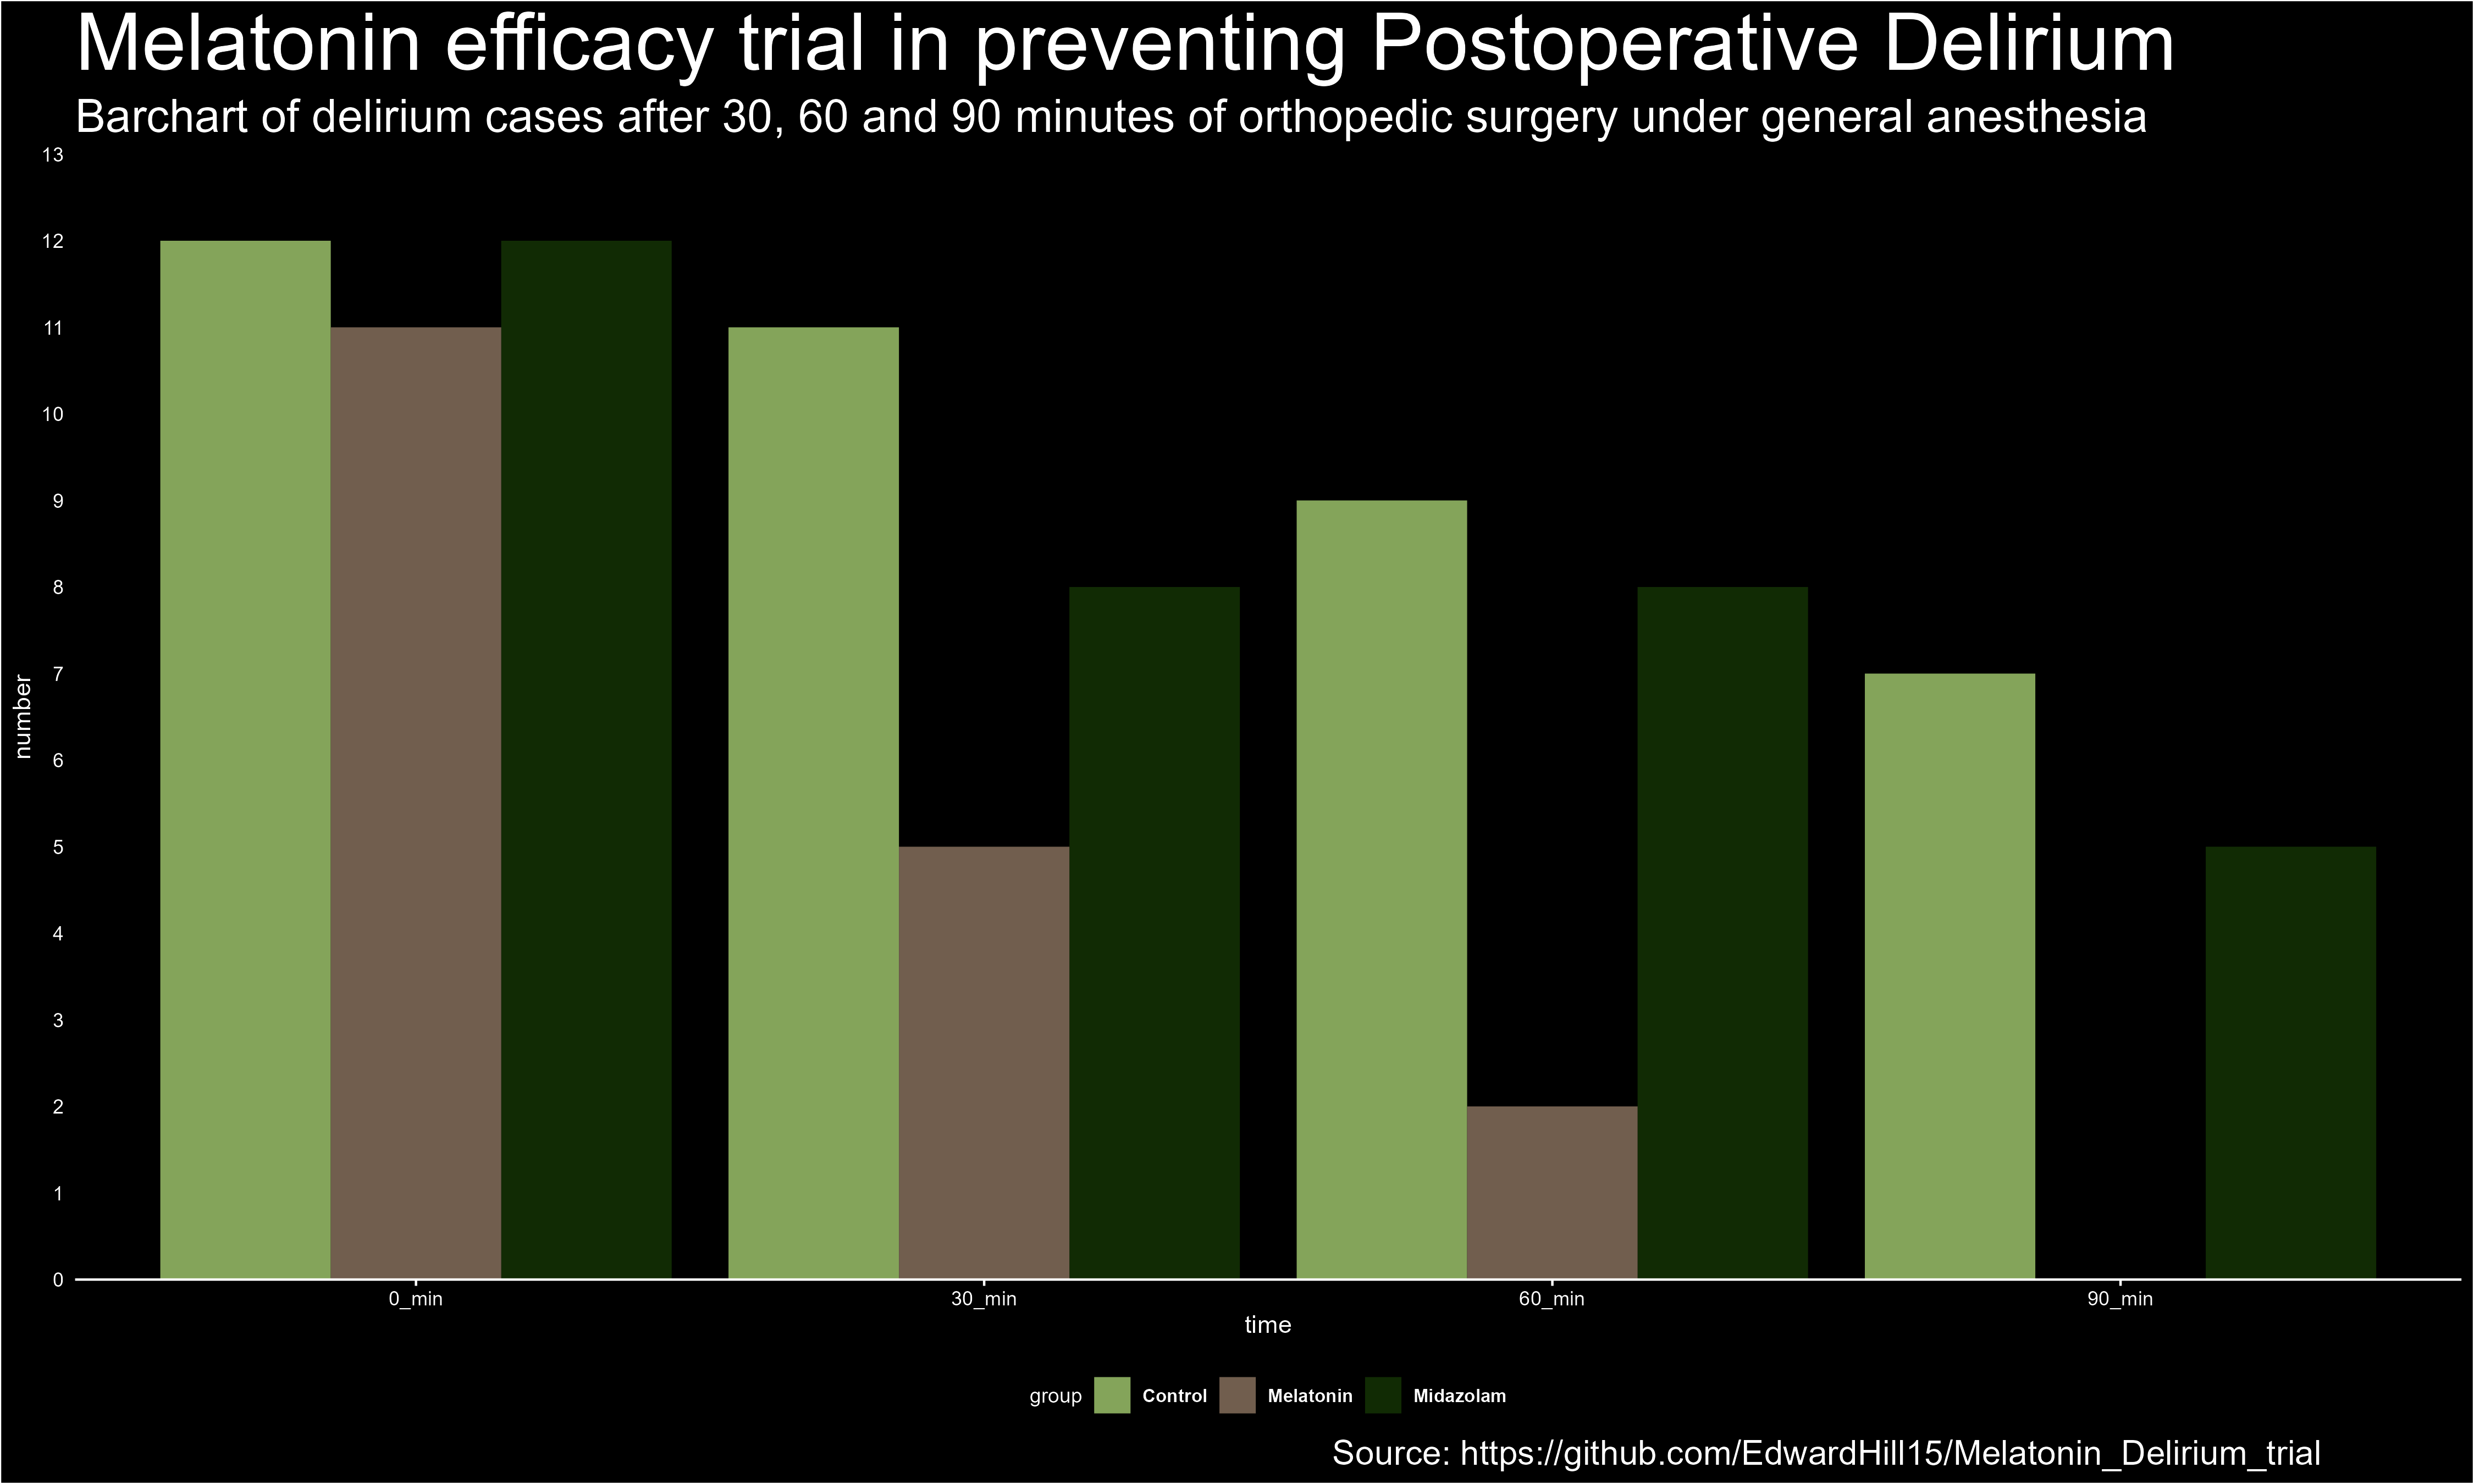
\includegraphics{https://raw.githubusercontent.com/EdwardHill15/Melatonin_Delirium_trial/main/plot_melatonin_delirium.png}
\caption{Bargraph of the Delirium-Melatonin study}
\end{figure}

\begin{verbatim}
## Rows: 3 Columns: 5
## -- Column specification --------------------------------------------------------
## Delimiter: ";"
## chr (1): group
## dbl (4): n0, n30, n60, n90
## 
## i Use `spec()` to retrieve the full column specification for this data.
## i Specify the column types or set `show_col_types = FALSE` to quiet this message.
\end{verbatim}

\begin{verbatim}
## [1] 3 5
\end{verbatim}

\begin{verbatim}
## 'data.frame':    3 obs. of  5 variables:
##  $ group: chr  "Control" "Midazolam" "Melatonin"
##  $ n0   : num  12 12 11
##  $ n30  : num  11 8 5
##  $ n60  : num  9 8 2
##  $ n90  : num  7 5 0
\end{verbatim}

\begin{verbatim}
##       group n0 n30 n60 n90
## 1   Control 12  11   9   7
## 2 Midazolam 12   8   8   5
## 3 Melatonin 11   5   2   0
\end{verbatim}

\begin{verbatim}
## 'data.frame':    12 obs. of  3 variables:
##  $ group : Factor w/ 3 levels "Control","Melatonin",..: 1 3 2 1 3 2 1 3 2 1 ...
##  $ time  : chr  "0_min" "0_min" "0_min" "30_min" ...
##  $ number: num  12 12 11 11 8 5 9 8 2 7 ...
\end{verbatim}

\hypertarget{odss-ratios-at-mdas-measurement-30-minutes-after-surgery}{%
\subsection{Odss ratios at MDAS measurement 30 minutes after
surgery}\label{odss-ratios-at-mdas-measurement-30-minutes-after-surgery}}

\begin{verbatim}
##           delirium30 non-delirium30
## melatonin          5              7
## control           11              1
\end{verbatim}

\begin{verbatim}
## 
##  Pearson's Chi-squared test with Yates' continuity correction
## 
## data:  table1a
## X-squared = 4.6875, df = 1, p-value = 0.03038
\end{verbatim}

\begin{verbatim}
##              Outcome +    Outcome -      Total               Prevalence *
## Exposed +            5            7         12     41.67 (15.17 to 72.33)
## Exposed -           11            1         12     91.67 (61.52 to 99.79)
## Total               16            8         24     66.67 (44.68 to 84.37)
## 
## Point estimates and 95% CIs:
## -------------------------------------------------------------------
## Prevalence ratio                               0.45 (0.23, 0.91)
## Odds ratio                                     0.06 (0.01, 0.68)
## Attrib prevalence in the exposed *             -50.00 (-81.98, -18.02)
## Attrib fraction in the exposed (%)            -120.00 (-338.99, -10.25)
## Attrib prevalence in the population *          -25.00 (-49.50, -0.50)
## Attrib fraction in the population (%)         -37.50 (-78.85, -5.71)
## -------------------------------------------------------------------
## Yates corrected chi2 test that OR = 1: chi2(1) = 4.688 Pr>chi2 = 0.030
## Fisher exact test that OR = 1: Pr>chi2 = 0.027
##  Wald confidence limits
##  CI: confidence interval
##  * Outcomes per 100 population units
\end{verbatim}

\begin{verbatim}
## 
##  Fisher's Exact Test for Count Data
## 
## data:  table1a
## p-value = 0.02719
## alternative hypothesis: true odds ratio is not equal to 1
## 95 percent confidence interval:
##  0.001331069 0.811072452
## sample estimates:
## odds ratio 
## 0.07377038
\end{verbatim}

\begin{verbatim}
##           delirium30 non-delirium30
## midazolam          8              4
## control           11              1
\end{verbatim}

\begin{verbatim}
## 
##  Pearson's Chi-squared test with Yates' continuity correction
## 
## data:  table1b
## X-squared = 1.0105, df = 1, p-value = 0.3148
\end{verbatim}

\begin{verbatim}
##              Outcome +    Outcome -      Total               Prevalence *
## Exposed +            8            4         12     66.67 (34.89 to 90.08)
## Exposed -           11            1         12     91.67 (61.52 to 99.79)
## Total               19            5         24     79.17 (57.85 to 92.87)
## 
## Point estimates and 95% CIs:
## -------------------------------------------------------------------
## Prevalence ratio                               0.73 (0.47, 1.12)
## Odds ratio                                     0.18 (0.02, 1.95)
## Attrib prevalence in the exposed *             -25.00 (-55.92, 5.92)
## Attrib fraction in the exposed (%)            -37.50 (-112.42, 10.99)
## Attrib prevalence in the population *          -12.50 (-35.05, 10.05)
## Attrib fraction in the population (%)         -15.79 (-40.54, 4.60)
## -------------------------------------------------------------------
## Yates corrected chi2 test that OR = 1: chi2(1) = 1.011 Pr>chi2 = 0.315
## Fisher exact test that OR = 1: Pr>chi2 = 0.317
##  Wald confidence limits
##  CI: confidence interval
##  * Outcomes per 100 population units
\end{verbatim}

\begin{verbatim}
## 
##  Fisher's Exact Test for Count Data
## 
## data:  table1b
## p-value = 0.3168
## alternative hypothesis: true odds ratio is not equal to 1
## 95 percent confidence interval:
##  0.003397033 2.472923285
## sample estimates:
## odds ratio 
##  0.1947795
\end{verbatim}

\begin{verbatim}
##           delirium30 non-delirium30
## melatonin          5              7
## midazolam          8              4
\end{verbatim}

\begin{verbatim}
## 
##  Pearson's Chi-squared test with Yates' continuity correction
## 
## data:  table1c
## X-squared = 0.67133, df = 1, p-value = 0.4126
\end{verbatim}

\begin{verbatim}
##              Outcome +    Outcome -      Total               Prevalence *
## Exposed +            5            7         12     41.67 (15.17 to 72.33)
## Exposed -            8            4         12     66.67 (34.89 to 90.08)
## Total               13           11         24     54.17 (32.82 to 74.45)
## 
## Point estimates and 95% CIs:
## -------------------------------------------------------------------
## Prevalence ratio                               0.63 (0.29, 1.36)
## Odds ratio                                     0.36 (0.07, 1.88)
## Attrib prevalence in the exposed *             -25.00 (-63.59, 13.59)
## Attrib fraction in the exposed (%)            -60.00 (-249.00, 26.65)
## Attrib prevalence in the population *          -12.50 (-45.80, 20.80)
## Attrib fraction in the population (%)         -23.08 (-68.45, 10.08)
## -------------------------------------------------------------------
## Uncorrected chi2 test that OR = 1: chi2(1) = 1.510 Pr>chi2 = 0.219
## Fisher exact test that OR = 1: Pr>chi2 = 0.414
##  Wald confidence limits
##  CI: confidence interval
##  * Outcomes per 100 population units
\end{verbatim}

\begin{verbatim}
## 
##  Fisher's Exact Test for Count Data
## 
## data:  table1c
## p-value = 0.4136
## alternative hypothesis: true odds ratio is not equal to 1
## 95 percent confidence interval:
##  0.04936444 2.44003372
## sample estimates:
## odds ratio 
##  0.3734813
\end{verbatim}

Table1a: melatonin vs control at 30 minutes: At 30 minutes after surgery
the \textbf{OR} was \textbf{0.06} with \textbf{95\%CI} of
\textbf{{[}0.01, 0.68{]}} when the \textbf{melatonin} group was compared
to the \textbf{control} group. That means that the pre-operative
administration of melatonin had a significant \textbf{(p = 0.030)}
\textbf{protective effect} on post-operative delirium state of
consciousness already 30 minutes after surgery.

Table1b: midazolam vs control at 30 minutes: At 30 minutes after surgery
the \textbf{OR} was \textbf{0.19} with \textbf{95\%CI} of
\textbf{{[}0.003, 2.473{]}} when the \textbf{midazolam} group was
compared to the \textbf{control} group. That means that the
pre-operative administration of midazolam had \textbf{not} a significant
\textbf{(p = 0.317)} \textbf{protective effect} on post-operative
delirium state of consciousness 30 minutes after surgery.

Table1c: melatonin vs midazolam at 30 minutes: At 30 minutes after
surgery the \textbf{OR} was \textbf{0.37} with \textbf{95\%CI} of
\textbf{{[}0.049, 2.440{]}} when the \textbf{melatonin} group was
compared to the \textbf{midazolam} group. That means that the
pre-operative administration of midazolam had \textbf{not} a significant
\textbf{(p = 0.414)} \textbf{protective effect} on post-operative
delirium state of consciousness 30 minutes after surgery.

\hypertarget{odds-ratios-at-mdas-measurement-60-minutes-after-surgery}{%
\subsection{Odds ratios at MDAS measurement 60 minutes after
surgery}\label{odds-ratios-at-mdas-measurement-60-minutes-after-surgery}}

\begin{verbatim}
##           delirium60 non-delirium60
## melatonin          2             10
## control            9              3
\end{verbatim}

\begin{verbatim}
## 
##  Pearson's Chi-squared test with Yates' continuity correction
## 
## data:  table2a
## X-squared = 6.042, df = 1, p-value = 0.01397
\end{verbatim}

\begin{verbatim}
##              Outcome +    Outcome -      Total               Prevalence *
## Exposed +            2           10         12      16.67 (2.09 to 48.41)
## Exposed -            9            3         12     75.00 (42.81 to 94.51)
## Total               11           13         24     45.83 (25.55 to 67.18)
## 
## Point estimates and 95% CIs:
## -------------------------------------------------------------------
## Prevalence ratio                               0.22 (0.06, 0.82)
## Odds ratio                                     0.07 (0.01, 0.49)
## Attrib prevalence in the exposed *             -58.33 (-90.66, -26.01)
## Attrib fraction in the exposed (%)            -350.00 (-1562.19, -21.83)
## Attrib prevalence in the population *          -29.17 (-60.75, 2.42)
## Attrib fraction in the population (%)         -63.64 (-131.80, -15.52)
## -------------------------------------------------------------------
## Uncorrected chi2 test that OR = 1: chi2(1) = 8.224 Pr>chi2 = 0.004
## Fisher exact test that OR = 1: Pr>chi2 = 0.012
##  Wald confidence limits
##  CI: confidence interval
##  * Outcomes per 100 population units
\end{verbatim}

\begin{verbatim}
## 
##  Fisher's Exact Test for Count Data
## 
## data:  table2a
## p-value = 0.01228
## alternative hypothesis: true odds ratio is not equal to 1
## 95 percent confidence interval:
##  0.005239828 0.647345444
## sample estimates:
## odds ratio 
## 0.07736941
\end{verbatim}

\begin{verbatim}
##           delirium60 non-delirium60
## midazolam          8              4
## control            9              3
\end{verbatim}

\begin{verbatim}
## Warning in chisq.test(table2b): Chi-squared approximation may be incorrect
\end{verbatim}

\begin{verbatim}
## 
##  Pearson's Chi-squared test with Yates' continuity correction
## 
## data:  table2b
## X-squared = 0, df = 1, p-value = 1
\end{verbatim}

\begin{verbatim}
##              Outcome +    Outcome -      Total               Prevalence *
## Exposed +            8            4         12     66.67 (34.89 to 90.08)
## Exposed -            9            3         12     75.00 (42.81 to 94.51)
## Total               17            7         24     70.83 (48.91 to 87.38)
## 
## Point estimates and 95% CIs:
## -------------------------------------------------------------------
## Prevalence ratio                               0.89 (0.53, 1.49)
## Odds ratio                                     0.67 (0.11, 3.93)
## Attrib prevalence in the exposed *             -8.33 (-44.55, 27.88)
## Attrib fraction in the exposed (%)            -12.50 (-88.57, 32.88)
## Attrib prevalence in the population *          -4.17 (-34.68, 26.34)
## Attrib fraction in the population (%)         -5.88 (-35.17, 17.06)
## -------------------------------------------------------------------
## Yates corrected chi2 test that OR = 1: chi2(1) = 0.000 Pr>chi2 = 1.000
## Fisher exact test that OR = 1: Pr>chi2 = 1.000
##  Wald confidence limits
##  CI: confidence interval
##  * Outcomes per 100 population units
\end{verbatim}

\begin{verbatim}
## 
##  Fisher's Exact Test for Count Data
## 
## data:  table2b
## p-value = 1
## alternative hypothesis: true odds ratio is not equal to 1
## 95 percent confidence interval:
##  0.07478974 5.44837199
## sample estimates:
## odds ratio 
##  0.6780693
\end{verbatim}

\begin{verbatim}
##           delirium60 non-delirium60
## melatonin          2             10
## midazolam          8              4
\end{verbatim}

\begin{verbatim}
## 
##  Pearson's Chi-squared test with Yates' continuity correction
## 
## data:  table2c
## X-squared = 4.2857, df = 1, p-value = 0.03843
\end{verbatim}

\begin{verbatim}
##              Outcome +    Outcome -      Total               Prevalence *
## Exposed +            2           10         12      16.67 (2.09 to 48.41)
## Exposed -            8            4         12     66.67 (34.89 to 90.08)
## Total               10           14         24     41.67 (22.11 to 63.36)
## 
## Point estimates and 95% CIs:
## -------------------------------------------------------------------
## Prevalence ratio                               0.25 (0.07, 0.94)
## Odds ratio                                     0.10 (0.01, 0.69)
## Attrib prevalence in the exposed *             -50.00 (-84.00, -16.00)
## Attrib fraction in the exposed (%)            -300.00 (-1407.74, -6.12)
## Attrib prevalence in the population *          -25.00 (-58.17, 8.17)
## Attrib fraction in the population (%)         -60.00 (-128.84, -11.87)
## -------------------------------------------------------------------
## Uncorrected chi2 test that OR = 1: chi2(1) = 6.171 Pr>chi2 = 0.013
## Fisher exact test that OR = 1: Pr>chi2 = 0.036
##  Wald confidence limits
##  CI: confidence interval
##  * Outcomes per 100 population units
\end{verbatim}

\begin{verbatim}
## 
##  Fisher's Exact Test for Count Data
## 
## data:  table2c
## p-value = 0.03607
## alternative hypothesis: true odds ratio is not equal to 1
## 95 percent confidence interval:
##  0.008101526 0.896925044
## sample estimates:
## odds ratio 
##  0.1121872
\end{verbatim}

Table2a: At 60 minutes after surgery the \textbf{OR} was \textbf{0.08}
with \textbf{95\%CI} of \textbf{{[}0.005, 0.647{]}} when the
\textbf{melatonin} group was compared to the \textbf{control} group.
That means that also after 60 minutes there is evidence for a
significant \textbf{protective effect} of pre-operative administration
of melatonin \textbf{(p = 0.012)} on post-operative delirium state of
consciousness.

Table2b: midazolam vs control at 60 minutes: At 60 minutes after surgery
the \textbf{OR} was \textbf{0.678} with \textbf{95\%CI} of
\textbf{{[}0.075, 5.448{]}} when the \textbf{midazolam} group was
compared to the \textbf{control} group. That means that the
pre-operative administration of midazolam had \textbf{not} a significant
\textbf{(p = 1.000)} \textbf{protective effect} on post-operative
delirium state of consciousness 60 minutes after surgery.

Table2c: melatonin vs midazolam at 60 minutes: At 60 minutes after
surgery the \textbf{OR} was \textbf{0.11} with \textbf{95\%CI} of
\textbf{{[}0.008, 0.897{]}} when the \textbf{melatonin} group was
compared to the \textbf{midazolam} group. That means that the
pre-operative administration of melatonin had a significant \textbf{(p =
0.036)} more \textbf{protective effect} on post-operative delirium state
of consciousness 60 minutes after surgery compared to the effect of
midazolam on it.

\hypertarget{odds-ratios-at-mdas-measurement-90-minutes-after-surgery}{%
\subsection{Odds ratios at MDAS measurement 90 minutes after
surgery}\label{odds-ratios-at-mdas-measurement-90-minutes-after-surgery}}

\begin{verbatim}
##           delirium90 non-delirium90
## melatonin          0             12
## control            7              5
\end{verbatim}

\begin{verbatim}
## 
##  Pearson's Chi-squared test with Yates' continuity correction
## 
## data:  table3a
## X-squared = 7.2605, df = 1, p-value = 0.007049
\end{verbatim}

\begin{verbatim}
##              Outcome +    Outcome -      Total               Prevalence *
## Exposed +            0           12         12       0.00 (0.00 to 26.46)
## Exposed -            7            5         12     58.33 (27.67 to 84.83)
## Total                7           17         24     29.17 (12.62 to 51.09)
## 
## Point estimates and 95% CIs:
## -------------------------------------------------------------------
## Prevalence ratio                               NaN (NaN, NaN)
## Odds ratio                                     NaN (NaN, NaN)
## Attrib prevalence in the exposed *             -58.33 (-86.23, -30.44)
## Attrib fraction in the exposed (%)            NaN (NaN, NaN)
## Attrib prevalence in the population *          -29.17 (-62.46, 4.13)
## Attrib fraction in the population (%)         -100.00 (-198.39, -34.05)
## -------------------------------------------------------------------
## Yates corrected chi2 test that OR = 1: chi2(1) = 7.261 Pr>chi2 = 0.007
## Fisher exact test that OR = 1: Pr>chi2 = 0.005
##  Wald confidence limits
##  CI: confidence interval
##  * Outcomes per 100 population units
\end{verbatim}

\begin{verbatim}
## 
##  Fisher's Exact Test for Count Data
## 
## data:  table3a
## p-value = 0.004577
## alternative hypothesis: true odds ratio is not equal to 1
## 95 percent confidence interval:
##  0.000000 0.449249
## sample estimates:
## odds ratio 
##          0
\end{verbatim}

\begin{verbatim}
##           delirium90 non-delirium90
## midazolam          5              7
## control            7              5
\end{verbatim}

\begin{verbatim}
## 
##  Pearson's Chi-squared test with Yates' continuity correction
## 
## data:  table3b
## X-squared = 0.16667, df = 1, p-value = 0.6831
\end{verbatim}

\begin{verbatim}
##              Outcome +    Outcome -      Total               Prevalence *
## Exposed +            5            7         12     41.67 (15.17 to 72.33)
## Exposed -            7            5         12     58.33 (27.67 to 84.83)
## Total               12           12         24     50.00 (29.12 to 70.88)
## 
## Point estimates and 95% CIs:
## -------------------------------------------------------------------
## Prevalence ratio                               0.71 (0.31, 1.63)
## Odds ratio                                     0.51 (0.10, 2.59)
## Attrib prevalence in the exposed *             -16.67 (-56.11, 22.78)
## Attrib fraction in the exposed (%)            -40.00 (-218.73, 38.51)
## Attrib prevalence in the population *          -8.33 (-42.66, 25.99)
## Attrib fraction in the population (%)         -16.67 (-65.43, 17.72)
## -------------------------------------------------------------------
## Uncorrected chi2 test that OR = 1: chi2(1) = 0.667 Pr>chi2 = 0.414
## Fisher exact test that OR = 1: Pr>chi2 = 0.684
##  Wald confidence limits
##  CI: confidence interval
##  * Outcomes per 100 population units
\end{verbatim}

\begin{verbatim}
## 
##  Fisher's Exact Test for Count Data
## 
## data:  table3b
## p-value = 0.6843
## alternative hypothesis: true odds ratio is not equal to 1
## 95 percent confidence interval:
##  0.07506651 3.35966548
## sample estimates:
## odds ratio 
##   0.524988
\end{verbatim}

\begin{verbatim}
##           delirium90 non-delirium90
## melatonin          0             12
## midazolam          5              7
\end{verbatim}

\begin{verbatim}
## 
##  Pearson's Chi-squared test with Yates' continuity correction
## 
## data:  table3c
## X-squared = 4.0421, df = 1, p-value = 0.04438
\end{verbatim}

\begin{verbatim}
##              Outcome +    Outcome -      Total               Prevalence *
## Exposed +            0           12         12       0.00 (0.00 to 26.46)
## Exposed -            5            7         12     41.67 (15.17 to 72.33)
## Total                5           19         24      20.83 (7.13 to 42.15)
## 
## Point estimates and 95% CIs:
## -------------------------------------------------------------------
## Prevalence ratio                               NaN (NaN, NaN)
## Odds ratio                                     NaN (NaN, NaN)
## Attrib prevalence in the exposed *             -41.67 (-69.56, -13.77)
## Attrib fraction in the exposed (%)            NaN (NaN, NaN)
## Attrib prevalence in the population *          -20.83 (-53.11, 11.45)
## Attrib fraction in the population (%)         -100.00 (-198.39, -34.05)
## -------------------------------------------------------------------
## Yates corrected chi2 test that OR = 1: chi2(1) = 4.042 Pr>chi2 = 0.044
## Fisher exact test that OR = 1: Pr>chi2 = 0.037
##  Wald confidence limits
##  CI: confidence interval
##  * Outcomes per 100 population units
\end{verbatim}

\begin{verbatim}
## 
##  Fisher's Exact Test for Count Data
## 
## data:  table3c
## p-value = 0.03727
## alternative hypothesis: true odds ratio is not equal to 1
## 95 percent confidence interval:
##  0.0000000 0.8864315
## sample estimates:
## odds ratio 
##          0
\end{verbatim}

Table3a: melatonin vs control at 90 minutes: At 90 minutes after surgery
the \textbf{OR} was \textbf{0} with \textbf{95\%CI} of \textbf{{[}0,
0.45{]}} when the \textbf{melatonin} group was compared to the
\textbf{control} group. That means that also after 90 minutes there is
evidence for a significant \textbf{protective effect} of pre-operative
administration of melatonin \textbf{(p = 0.005)} on post-operative
delirium state of consciousness.

Table3b: midazolam vs control at 90 minutes: At 90 minutes after surgery
the \textbf{OR} was \textbf{0.525} with \textbf{95\%CI} of
\textbf{{[}0.075, 3.360{]}} when the \textbf{midazolam} group was
compared to the \textbf{control} group. That means that the
pre-operative administration of midazolam had \textbf{not} a significant
\textbf{(p = 0.684)} \textbf{protective effect} on post-operative
delirium state of consciousness 90 minutes after surgery.

Table3c: melatonin vs midazolam at 90 minutes: At 90 minutes after
surgery the \textbf{OR} was \textbf{0} with \textbf{95\%CI} of
\textbf{{[}0, 0.886{]}} when the \textbf{melatonin} group was compared
to the \textbf{midazolam} group. That means that the pre-operative
administration of melatonin had a significant \textbf{(p = 0.037)} more
\textbf{protective effect} on post-operative delirium state of
consciousness 90 minutes after surgery compared to the effect of
midazolam on it.

\hypertarget{chi-squared-test-for-the-total-group-n36}{%
\subsection{Chi Squared Test for the Total Group
(N=36)}\label{chi-squared-test-for-the-total-group-n36}}

\begin{verbatim}
##           delirium non-delirium
## control          7            5
## midazolam        5            7
## melatonin        0           12
\end{verbatim}

\begin{verbatim}
## 
##  Pearson's Chi-squared test
## 
## data:  table_x2
## X-squared = 9.75, df = 2, p-value = 0.007635
\end{verbatim}

\hypertarget{results-chi-squared-test-total-group}{%
\subsection{Results Chi-Squared Test Total
Group:}\label{results-chi-squared-test-total-group}}

The results of the Pearson's Chi-squaerd test of \textbf{\emph{X2}} (2,
\textbf{\emph{N}} = 36) = 9.75, \textbf{\emph{p}} = \textbf{.0076}
indicate that the pre-operative administration of melatonin is
\textbf{dependent} on the outcome, i.e., the prevalence of a
post-operative state of delirium after surgery. That means that the
pre-operative administration of melatonin had a \textbf{significant}
effect on reducing a post-operative state of delirium after surgery.

\hypertarget{summary-results-of-reviewers-analyses}{%
\subsection{Summary results of reviewer's
analyses}\label{summary-results-of-reviewers-analyses}}

These results are related to odds ratios (OR) at MDAS (Memorial Delirium
Assessment Scale) measurement 30 minutes after surgery.

In Table1a, the comparison was made between the melatonin group and the
control group. The OR was found to be 0.06, with a 95\% confidence
interval (CI) of {[}0.01, 0.68{]}. This means that the pre-operative
administration of melatonin had a significant protective effect (p =
0.030) on post-operative delirium state of consciousness already 30
minutes after surgery.

In Table1b, the comparison was made between the midazolam group and the
control group. The OR was found to be 0.19, with a 95\% CI of {[}0.003,
2.473{]}. This means that the pre-operative administration of midazolam
did not have a significant (p = 0.317) protective effect on
post-operative delirium state of consciousness 30 minutes after surgery.

In Table1c, the comparison was made between the melatonin group and the
midazolam group. The OR was found to be 0.37, with a 95\% CI of
{[}0.049, 2.440{]}. This means that the pre-operative administration of
melatonin did not have a significant (p = 0.414) protective effect on
post-operative delirium state of consciousness 30 minutes after surgery
compared to the effect of midazolam on it.

At 60 minutes after surgery, there is evidence for a significant
protective effect of pre-operative administration of melatonin (p =
0.012) on post-operative delirium state of consciousness. However, the
pre-operative administration of midazolam had no significant protective
effect (p = 1.000) on post-operative delirium state of consciousness 60
minutes after surgery.

Additionally, the pre-operative administration of melatonin had a
significant (p = 0.036) more protective effect on post-operative
delirium state of consciousness 60 minutes after surgery compared to the
effect of midazolam on it.

At 90 minutes after surgery, the odds ratio (OR) for the melatonin group
compared to the control group was 0 with a 95\% confidence interval (CI)
of {[}0, 0.45{]}, indicating a significant protective effect of
pre-operative melatonin administration on post-operative delirium state
of consciousness (p = 0.005). However, for the midazolam group compared
to the control group, the OR was 0.525 with a 95\% CI of {[}0.075,
3.360{]}, suggesting that pre-operative administration of midazolam did
not have a significant protective effect on post-operative delirium
state of consciousness (p = 0.684) at 90 minutes after surgery.
Additionally, when comparing the melatonin and midazolam groups, the OR
was 0 with a 95\% CI of {[}0, 0.886{]}, indicating that pre-operative
melatonin had a significantly more protective effect (p = 0.037) on
post-operative delirium state of consciousness at 90 minutes after
surgery compared to the effect of midazolam.

Finally, a Chi-squared test showed that the administration of melatonin
had a significant effect on reducing post-operative delirium. These
findings suggest that pre-operative administration of melatonin may be
an effective way to prevent post-operative delirium in patients.

\hypertarget{conclusion}{%
\subsection{Conclusion}\label{conclusion}}

Based on the results, it can be concluded that pre-operative
administration of melatonin has a significant protective effect on
post-operative delirium state of consciousness. This effect was observed
as early as 30 minutes after surgery and continued up to 90 minutes
after surgery. On the other hand, pre-operative administration of
midazolam did not show a significant protective effect on post-operative
delirium state of consciousness at any of the measurement times.

Furthermore, when comparing the effect of melatonin to midazolam,
melatonin was found to be significantly more effective in protecting
against post-operative delirium state of consciousness at both 60 and 90
minutes after surgery.

These findings suggest that melatonin may be a promising option for
preventing post-operative delirium state of consciousness, while
midazolam may not provide significant benefits in this regard. However,
further studies are needed to confirm these findings and to evaluate the
long-term effects of melatonin on post-operative delirium state of
consciousness.

\hypertarget{discussion}{%
\subsection{Discussion}\label{discussion}}

The results of this study suggest that pre-operative administration of
melatonin has a significant protective effect on post-operative delirium
state of consciousness, whereas pre-operative administration of
midazolam did not show a significant protective effect. This effect was
observed as early as 30 minutes after surgery and remained significant
at 60 and 90 minutes after surgery. Additionally, the protective effect
of melatonin was found to be significantly stronger than that of
midazolam at 60 and 90 minutes after surgery.

These findings have important clinical implications, as post-operative
delirium is a common complication of surgery, especially in elderly
patients, and can lead to increased morbidity and mortality. Melatonin,
as a natural hormone with sedative and antioxidant properties, may be a
safer and more effective alternative to traditional sedatives like
midazolam for preventing post-operative delirium.

However, it is important to note that this study has some limitations,
including the small sample size and the use of only one dose of
melatonin and midazolam. Further research with larger sample sizes and
more doses of melatonin and midazolam is needed to confirm these
findings and to explore the optimal dose and timing of administration
for maximum effect.

In conclusion, the findings of this study suggest that pre-operative
administration of melatonin may be an effective way to prevent
post-operative delirium, and may be a safer alternative to traditional
sedatives. However, further research is needed to confirm these findings
and to explore the optimal dose and timing of administration.

\end{document}
